\documentclass{beamer}

\usepackage{amsmath}
% \usepackage{dingbat}
\usepackage{twemojis}
\usepackage{xspace}

\input{../../papers/macros/style.tex}
\input{../../papers/macros/primitives.tex}

\def\comring{\ensuremath{\mathsf{comring}}\xspace}
\def\compk{\ensuremath{\mathsf{compk}}\xspace}


\title{Ethical identity, ring VRFs, and \\ zero-knowledge continuations}

\author{Jeffrey Burdges \and Handan Kilinc-Alper \and Alistair Stewart \and Sergey Vasilyev}
\date{16-17 May 2024 \\ \vphantom{|} \\ \vphantom{|} \\ \url{https://eprint.iacr.org/2022/002} \\ \url{https://github.com/w3f/ring-vrf/}}




\begin{document}


\maketitle


% \end{frame}
% \bigskip % \bigskip
% \begin{frame}



\begin{frame}
	
Ring signatures prove the actual signer exists in \\
\hspace{10pt} some publicly specified list, known as the ring.

\bigskip\bigskip

Examples:  Some ``deniable'' key exchanges, Monero, ZCash, etc.

\bigskip\bigskip

Ring can be a fancy set commitment like ZCash, \\
\hspace{10pt} but membership proofs are always very expensive.
	
\end{frame}



\begin{frame}{EC VRF}

A verifiable random function (VRF) proves evaluation of a pseudo-random function (PRF) determined by a signing key.

\bigskip\bigskip

$\mathsf{ECVRF}.\Verify(\msg,\aux,\pk,(\Out,R,R_\msg,s))$
	
$$ \begin{aligned}
\In &:= H_{\mathcal{G}}(\msg) \\
c &:= H(\msg,\aux,\pk,\Out,R,R_\msg) \\
s \, \In &== c \, \Out + R_\msg \\
s \, G &== c \, \pk + R \\
& \mathtt{return}\, H(\Out,\msg) \\
\end{aligned} $$
	
\end{frame}



\begin{frame}

Ring VRF is a ring signature that's also a VRF.

\bigskip\bigskip 

A ring verifiable random function (ring VRF) is a ring signature that proves evaluation of a pseudo-random function (PRF) determined by the actual key pair.

\end{frame}



\begin{frame}

For what do you use a ring VRF?

\bigskip\bigskip

% black_FRONT050.png

\begin{columns}
        \begin{column}[t]{0.1\textwidth}
        \end{column}
        \begin{column}[t]{0.3\textwidth}
                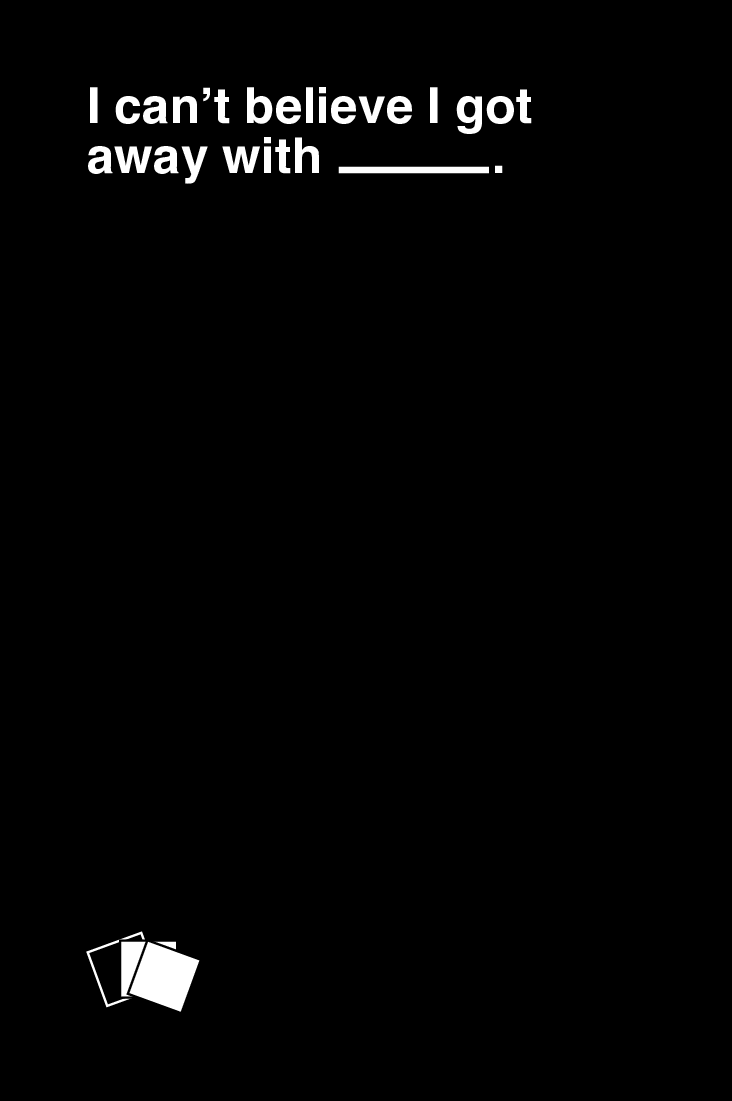
\includegraphics[width=.9\textwidth]{../images/black_FRONT012.png} % {CAC/PNGs-to-print/individual-cards/black_FRONT012.png}
        \end{column}
        \begin{column}[t]{0.3\textwidth}
                \frame{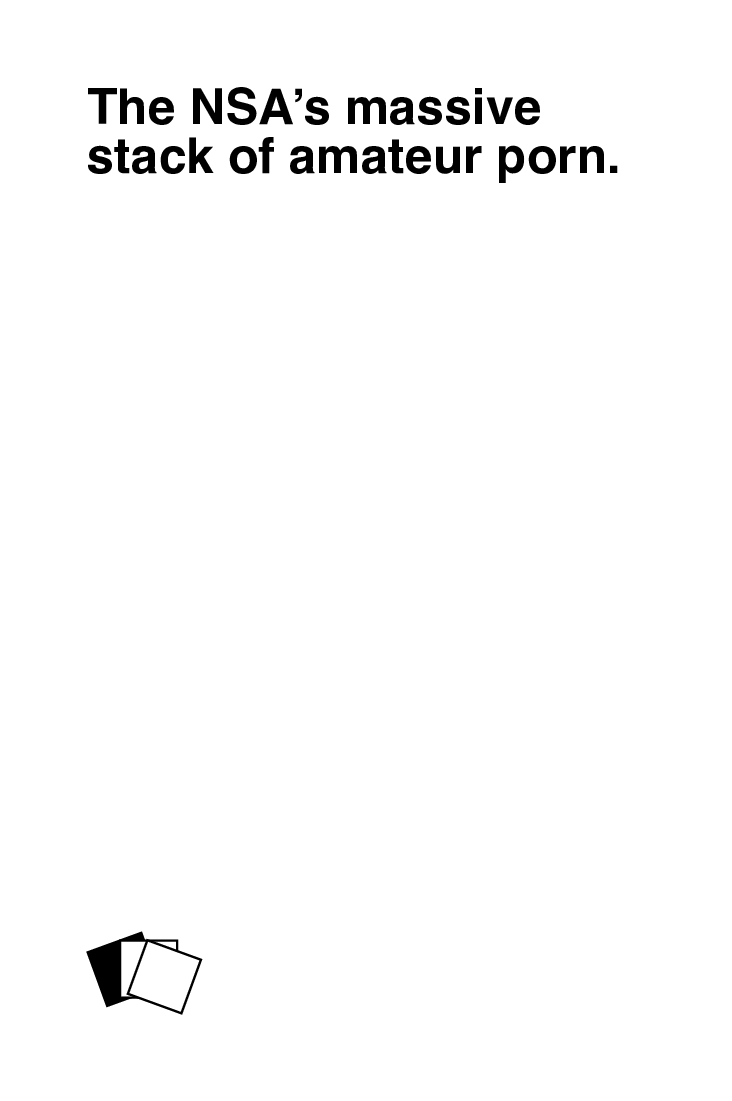
\includegraphics[width=.9\textwidth]{../images/white_FRONT227.png}} % {CAC/PNGs-to-print/individual-cards/white_FRONT227.png}
        \end{column}
        \begin{column}[t]{0.3\textwidth}
            \frame{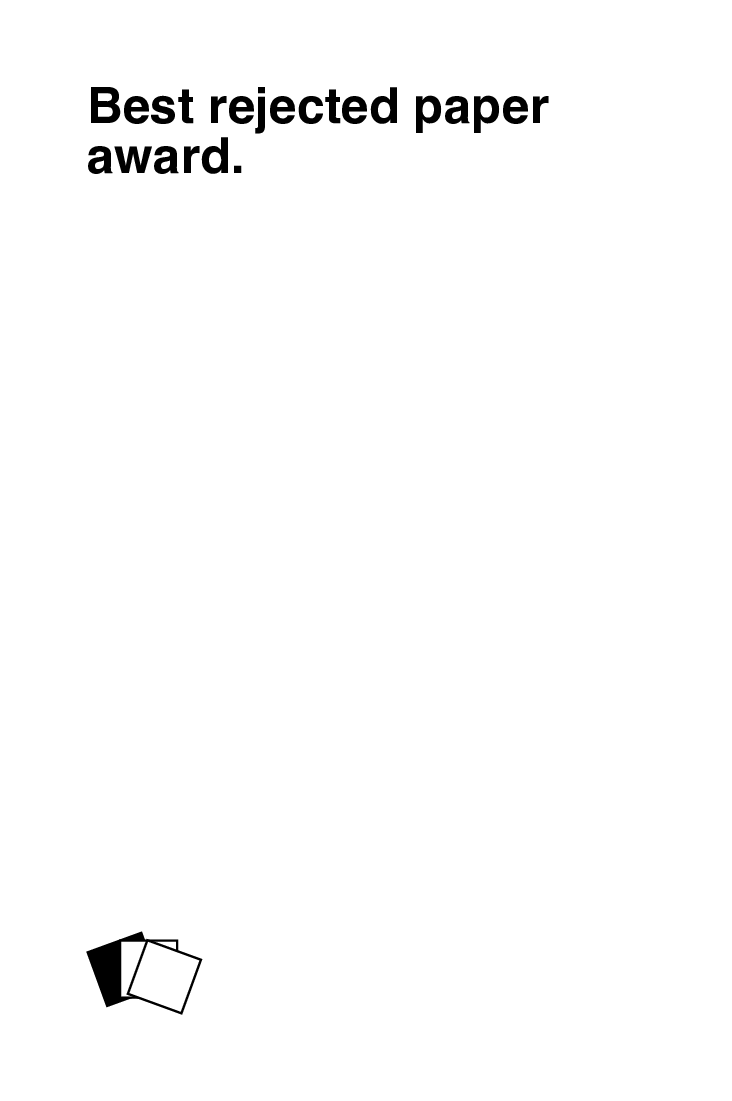
\includegraphics[width=.9\textwidth]{../images/white_FRONT117.png}} % {CAC/PNGs-to-print/individual-cards/black_FRONT050.png}
    \end{column}
\end{columns}

\end{frame}



\begin{frame}{Pedersen VRF}

We set $\compk := \sk \, G + {\color{red} b \, K}$ to be a Pedersen commitment to $\sk$.

\bigskip\bigskip

$\mathsf{PedersenVRF}.\Verify(\msg,\aux,\compk,(\Out,R,R_\msg,s,{\color{red} t}))$
	
$$ \begin{aligned}
\In &:= H_{\mathcal{G}}(\msg) \\
c &:= H(\msg,\aux,\compk,\Out,R,R_\msg) \\
s \, \In &== c \, \Out + R_\msg \\
{\color{red} t \, K} + s \, G &== c \, \compk + R \\
& \mathtt{return} \, H(\Out,\msg) \\
\end{aligned} $$

\bigskip \bigskip

Just EC VRF except for $\color{red} t, b$ and $\pk$ being $\compk$.

\end{frame}



\begin{frame}
	
Zero-knowledge continuations..
	
\bigskip
	
Q: What are the fastest/cheapest SNARK proofs?
	
\bigskip
	
A: Ones we reuse without reproving.
	
\end{frame}


\begin{frame}[t] % {Zero-knowledge continuations}

$\mathsf{Groth16}.\Verify(X,(A,B,C))$

$$ e(A,B) = e([\alpha]_1, [\beta]_2) \cdot e(X, [\gamma]_2) \cdot e(C, [\delta]_2) $$

\pause\medskip

$$ \begin{aligned}
 X &= \sk \, G + \comring \, L \\
\end{aligned} $$

\vspace{-10pt}
$$ \mathsf{Groth16} \Setst{ \sk, \comring \vphantom{\big|} }{
\begin{aligned}
  \exists d \textrm{\ s.t.\ } \pk &\leftarrow \mathsf{Posideon}(sk,d) \\
  \exists o \textrm{\ s.t.\ } \pk &\in_o \comring \\
\end{aligned}
%    \exists d,o \textrm{\ s.t.\ } \mathsf{Posideon}(sk,d) \in_o \comring 
} $$

\pause\bigskip\bigskip\bigskip 

% \hspace{10pt}
{\it Special(ized) G(roth16) means inner Groth16 leaks secrets, but..}

\end{frame}


\begin{frame}[t] % {Zero-knowledge continuations}

$\mathsf{Groth16}.\Verify(X,(A,B,C))$

$$ e(A,B) = e([\alpha]_1, [\beta]_2) \cdot e(X, [\gamma]_2) \cdot e(C, [\delta]_2) $$

\smallskip

$$ \begin{alignedat}{2}
 X &= \sk \, G + {\color{red} b \, K} &&+ \, \comring \, L \\
   &= \, \, \, \, \compk  &&+ \, \comring \, L \\
\end{alignedat} $$

\bigskip

Add $\color{red} K_\delta := {\gamma\over\delta} K$ to trusted setup

$$ \begin{aligned}
X' &:= X + {\color{red} b\, K} &\quad&&
B' &:= r_1 B + r_1 r_2 [\delta]_2 \\
A' &:= {1 \over r_1} A & &&
C' &:= C + r_2 A + {\color{red} b\, K_\delta} \\
\end{aligned} $$

\bigskip\bigskip

\hspace{5pt} Marginal signer cost of eight $\mathcal{G}_1$ mults plus two $\mathcal{G}_2$ mults \quad {\Large\twemoji{tada}}

% \pause\bigskip\medskip
% \hspace{30pt} {\it Welcome to zero-knowledge continuations \quad {\Large\twemoji{tada}}}

\end{frame}



% \begin{frame}
% \end{frame}
% \pause\bigskip\bigskip 



\begin{frame} % {Identity}
	
Q: How can identity be safe for online use?

\bigskip

A: By revealing nothing except users' uniqueness.

\bigskip\bigskip

\hspace{10pt} No W3C attribute based bullshit!

\end{frame}



\begin{frame} % {Identity}

Attribute credentials signed by authority.

\bigskip\smallskip

User agent: \\ \smallskip

- Validates TLS cert of ``site.com'' \\ \smallskip
- Gets attribute request: name, age, nationality, employment status \\ \smallskip
\only<2>{{\color{red} - Validates DPA certificate for attributes at ``site.com''} \\ \smallskip}
- Asks user to approve sharing those attributes with ``site.com''. \\
\hspace{10pt} If approved, proves the atttributes

\bigskip\smallskip

Issues: \\ \smallskip

% - Authorities issue fraudulent certificates, ala CAs and Covid. \\ \small
- Attributes are unecessarily invasive. \\ \smallskip
- Attributes leak across domains.  Users cannot change attributes. \\ \smallskip
- Users make mistakes and/or can be forced. \\ \medskip
\hspace{30pt}  \only<2>{{\color{red} Attribute requests need certificate infrastructure.}}

\end{frame}



\begin{frame} % {Identity}

Ring consists of people, with one key per person, \\ 
\hspace{10pt} maybe populated from government identity documents.

\bigskip\smallskip

User agent: \\ \smallskip

1st) validates TLS cert of ``site.com'', including CT logs. \\ \smallskip

2nd) sends ring VRF signature with $\msg = \mathtt{``site.com``}$. \\ \smallskip

\pause\bigskip\bigskip 

Do we have a ``right to be forgotten'' at ``site.com``? \\ \smallskip

\hspace{10pt} If so, use $\msg = \mathtt{``site.com``} \doubleplus \mathsf{month}$

\end{frame}



\begin{frame}

Q: Can ring VRFs give us efficent anonymous payments?

\bigskip

A: Not really, but they can give anonymous rate limiting

\end{frame}



\begin{frame}

``No civilization can possibly survive to an interstellar spacefaring \\ \smallskip
\hspace{1pt} phase unless it limits its numbers'' (and its consumption) \\ \medskip
\hspace{1pt} --- Carl Sagan

\bigskip\bigskip 

We're headed for $+4^{\circ}$C by 2100, so uninhabitable tropics \\
\hspace{10pt} and world carrying capacity below 1 billion people (Steffan). \\ \bigskip

50\% odds ``of a synchronous crop failure [$>10$\%] across all four [major maize producing] countries during 2040s''~(Chatham~House) \\

\end{frame}



\begin{frame}

Anonymous rationing uses $\msg = \mathtt{``moutarde``} \doubleplus \mathsf{week} \doubleplus \mathsf{counter}$ \\
\hspace{1pt} And treats outputs as short lived nullifiers.

\bigskip\bigskip 

Also yields free-to-play games, promotional discounts, etc.

\end{frame}



\begin{frame}

As fraudulent TLS and covid certificates are commonplace..

\bigskip

Q: How can ration cards be trusted?

\bigskip 

A: By asking users trust a public list of residents, not certificates.

% Important: Ring membership can be transparent!  No fraudulent certificates!

\end{frame}



\begin{frame}{Sassafras}

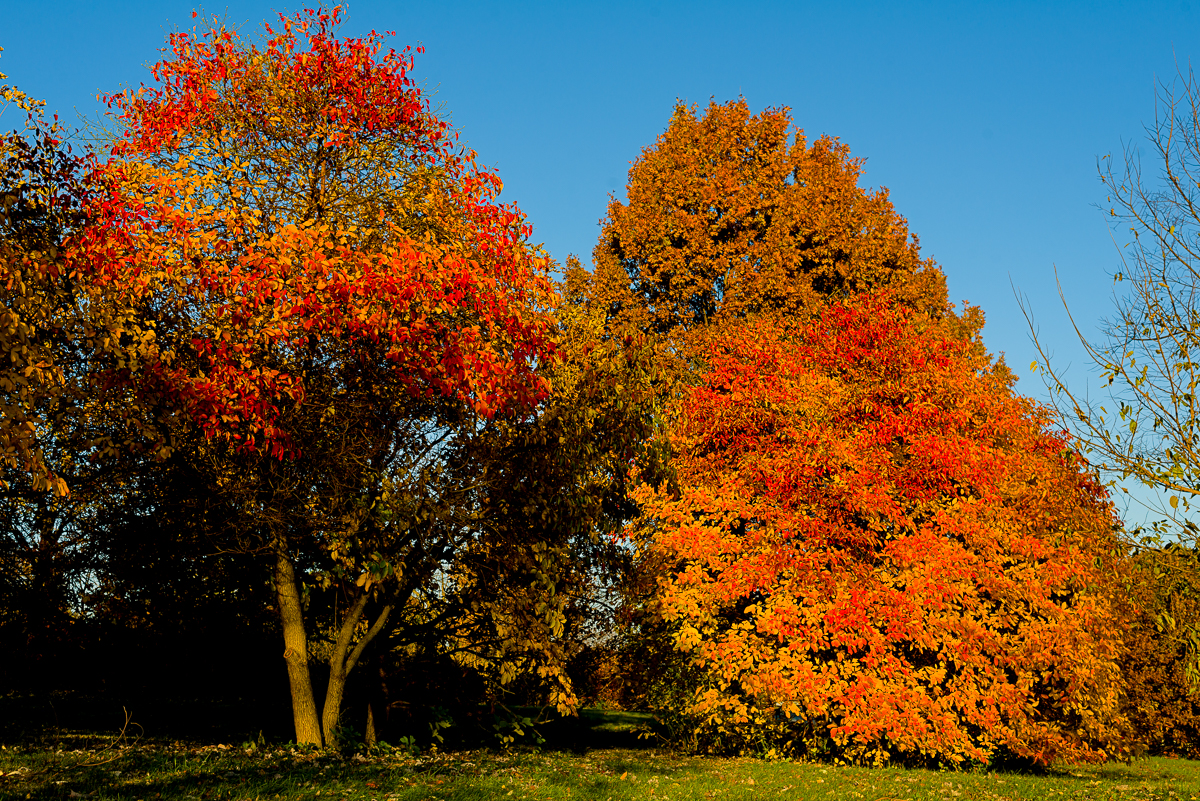
\includegraphics[width=\textwidth]{../images/Sassafras-albidum.jpg}

\end{frame}



\begin{frame}

Sassafras: Semi-anonymous sortition of staked assignees \\
\hspace{5pt} for fixed-time rhythmic assignment of slots

\bigskip

It's a (semi) secret single leader election (semi-SSLE) \\
\hspace{5pt} by cards against humanity.

\bigskip

% black_FRONT050.png

\begin{columns}
	\begin{column}[t]{0.1\textwidth}
	\end{column}
	\begin{column}[t]{0.3\textwidth}
		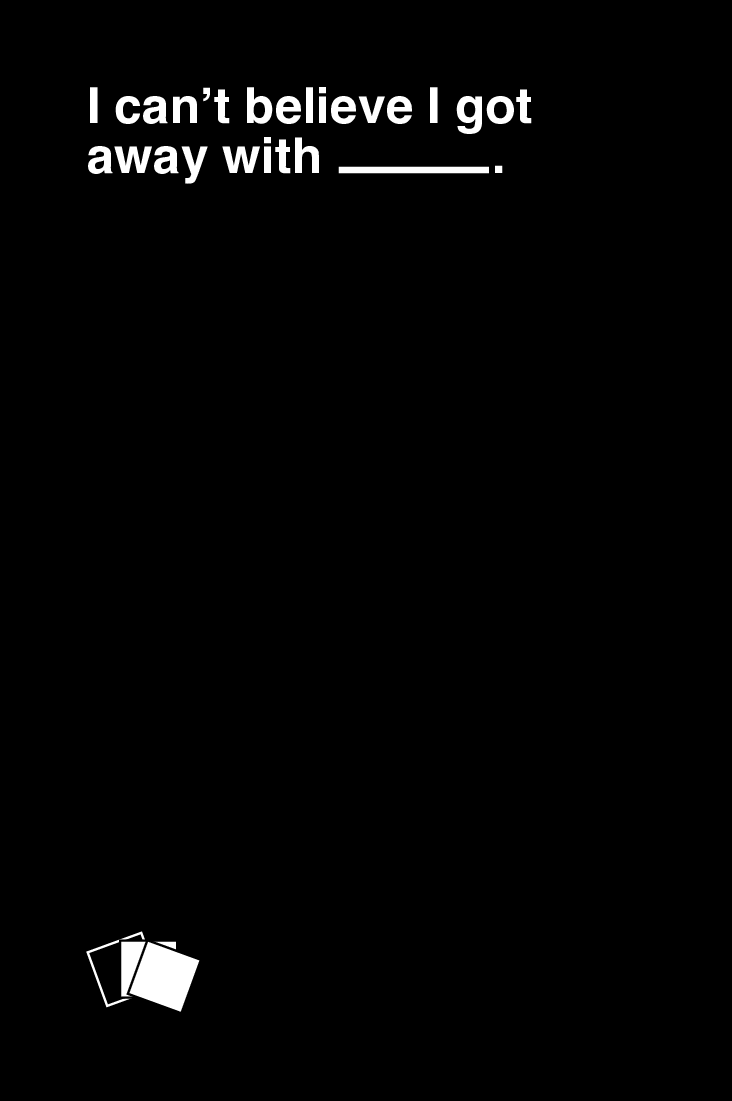
\includegraphics[width=.9\textwidth]{../images/black_FRONT012.png} % {CAC/PNGs-to-print/individual-cards/black_FRONT012.png}
	\end{column}
	\begin{column}[t]{0.3\textwidth}
		\frame{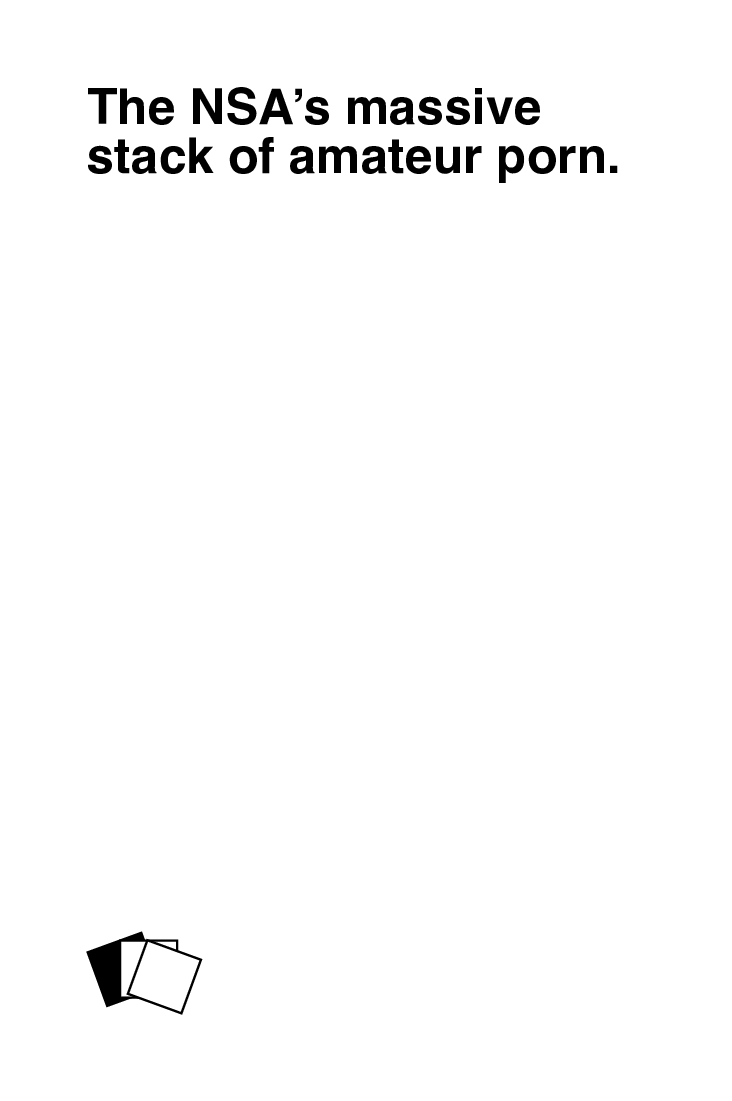
\includegraphics[width=.9\textwidth]{../images/white_FRONT227.png}} % {CAC/PNGs-to-print/individual-cards/white_FRONT227.png}
	\end{column}
	\begin{column}[t]{0.3\textwidth}
	    \frame{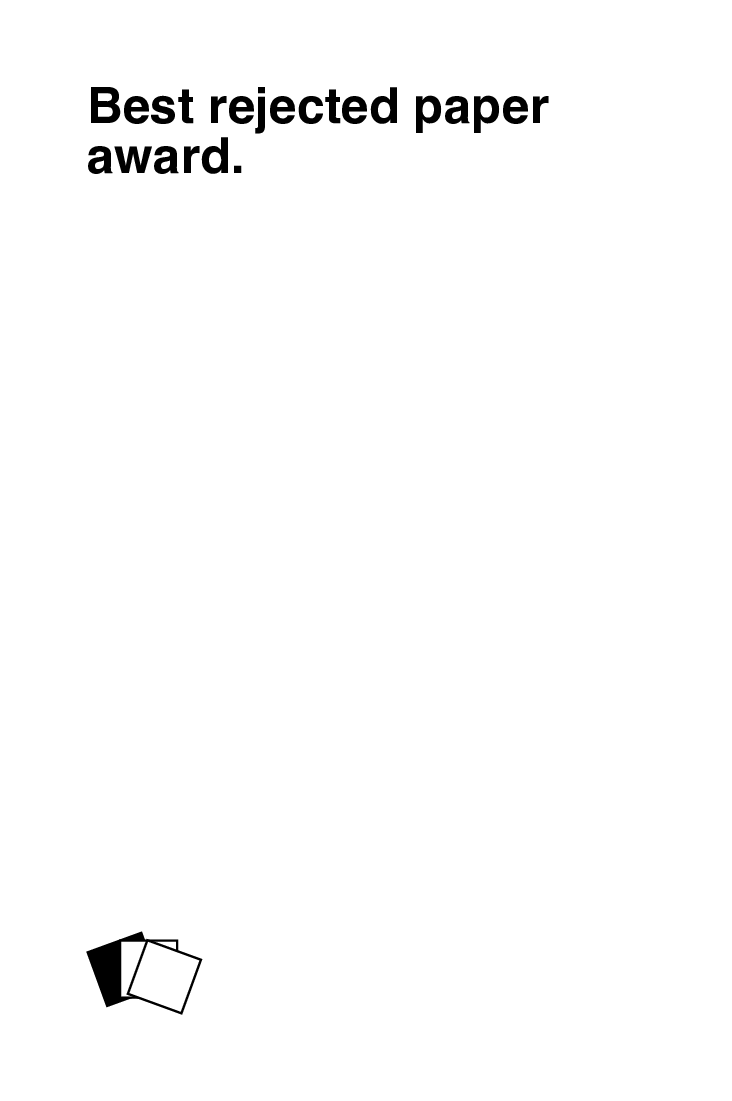
\includegraphics[width=.9\textwidth]{../images/white_FRONT117.png}} % {CAC/PNGs-to-print/individual-cards/black_FRONT050.png}
    \end{column}
\end{columns}


\end{frame}



\begin{frame}{Sassafras}

Disadvantages: \\
- Network layer anonymity is weak, but we care little.. \\

\bigskip\bigskip

Advantages: \\ \smallskip
- Ouroboros Praos quality randomness \\ \smallskip
- Vastly more efficient than Boneh's shuffle SSLEs \\ \smallskip
- Block producers can prove their slot in advance \\ \smallskip
- Users send tx to upcoming slots via Tor-like {.onion} circuits. \\ \smallskip
% Tor-like {.onion} circuit to upcoming slots \\
%  \hspace{5pt} so users can sent tx directly to upcoming slots. \\ \smallskip
- Avoids need for memepools, saving bandwidth and CPU. \\ \smallskip
- Better MEV defenses \\ \smallskip

\end{frame}




\begin{frame}{Zero-knowledge in substrate?}

Yes WASM works, but 10x slower for some optimized code.

\bigskip \bigskip

EIP-2537 (BLS12-381) adds 9 precompiles (hostcalls).  
{\Large\twemoji{thumbs down}}
% 
\includegraphics[width=0.03\textwidth]{../images/thumbs_down.png}
\\ \medskip

\only<1>{
\hspace{5pt} Extra complexity means fewer curves \\
\hspace{10pt}- Addition \& hash-to-curve appear unecessary. \\ \medskip

\hspace{5pt} Inflexibility yields worse performance  \\ 
\hspace{10pt}- Groth16 needs 4 pairings \\
\hspace{10pt}- Batch verifiers \\
\hspace{10pt}- Large parameters like KZG trusted setups \\
}
\bigskip\bigskip
\only<2>{
Add hostcalls for the "slow parts" but use WASM elsewhere
{\Large\twemoji{thumbs up}}
% 
\includegraphics[width=0.03\textwidth]{../images/thumbs_up.png}
\\ \smallskip

\hspace{5pt} Bandersnatch, etc. --- single \& multi-scalar multiplication \\

\hspace{5pt} BLS12-381, BLS12-377, BW6-761, BW6-767, BN254 --- \\
\hspace{10pt}  Same, plus multi-miller loop \& final exponentiation \\ \smallskip
}

\bigskip \bigskip 

\url{https://github.com/paritytech/arkworks-extensions}
\end{frame}


\begin{frame}

Arkworks \& others mostly descend from Zcash. \\ \smallskip

Adapt crates directly, without reimplementation.

\smallskip

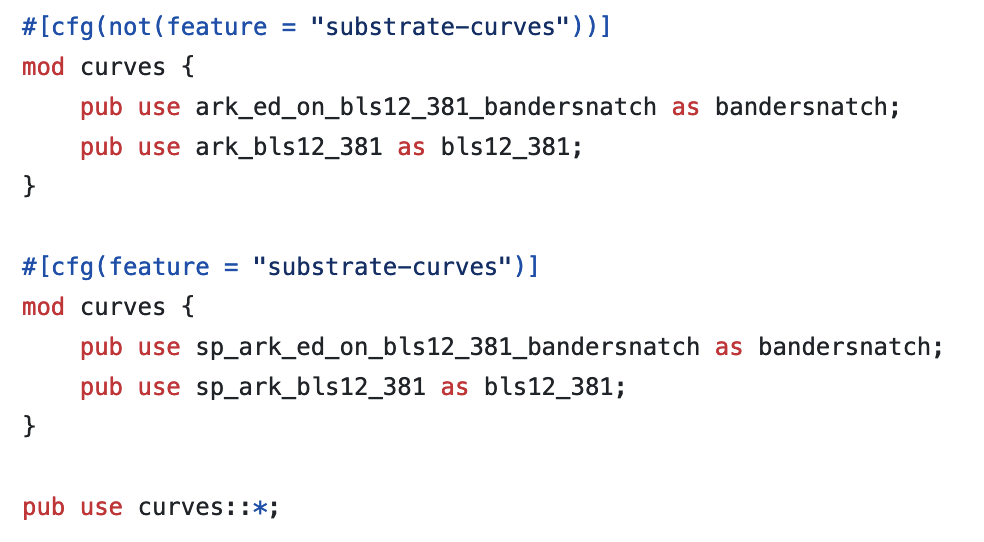
\includegraphics[width=0.9\textwidth]{../images/use_curves.png}

\url{https://github.com/paritytech/arkworks-extensions}

\end{frame}



\end{document}





\begin{frame}
		
\end{frame}



\begin{frame}
	
\end{frame}





\begin{frame} % {Zero-knowledge continuations}

\hspace{30pt} {\it Are there other zero-knowledge continuations?}

\bigskip\medskip

Avoid the Groth16 side channel and use CDH over Posideon.. \\ \smallskip

\bigskip\medskip

$$ X = \sk \, G + b \, K + J_\pk.x \, L_x + J_\pk.y \, L_y $$

\vspace{-20pt}
$$ \mathsf{Groth16} \Setst{ \sk_0 + \sk_1 2^{128}, J_\pk }{ 
	\exists d \textrm{\ s.t.\ }
	J_\pk = \sk_0 J_0 + \sk_1 J_1 + d J_2
} $$

\smallskip

Use with hidden KZG opening of $J_\pk$ like Caulk/Caulk+

\end{frame}


\begin{frame} % {Zero-knowledge continuations}

Revokation could be done using a ``cuckoo filter'' in a KZG.

$$ \mathsf{Groth16} \Setst{ \sk, \pk, i_1, i_2, i_3, \comring \vphantom{\big|} }{
\begin{aligned}
  \exists d \textrm{\ s.t.\ } \pk &\leftarrow \mathsf{Posideon}(sk,d) \\
  \exists o \textrm{\ s.t.\ } \pk &\in_o \comring \\
  (i_1,i_2,i_3) &\leftarrow \mathsf{Posideon}(pk) \\
\end{aligned}
} $$

\smallskip

Non-revokation proof:  $\pk \neq f(i_j)$ for $j=1,2,3$ where $f$ is a KZG
\hspace{10pt} Nolonger like Caulk/Caulk+.

\end{frame}


